\section{Issues}
The project did not go as smoothly as we had hoped. The group agreed on pretty much everything, but the issues we had were mostly related to the software and tools not cooperating or working as we expected.

\subsection{C\# Compiler}
When we tried to add the database to our project via the Entity Framework we had troubles with the C\# compiler not being found. This was due to the installation of the Visual Studio 2012 Release Candidate edition (which had expired), so we had to uninstall this RC version to install the "normal" Visual Studio 2012 which lead to the compiler not working - we couldn't add new items, compile or make a new project.

There was however a quickfix to repair the compiler by using the gacutil utility software included with Visual Studio 2012.
This command in cmd fixed it:
\begin{verbatim}
gacutil /u Microsoft.VisualStudio.CSharp.Services.Language.Interop 
\end{verbatim}

\subsection{GitHub DDoS}
On October 14, the day of the midterm delivery, GitHub experienced a DDoS attack. This resulted in some of the files we were working on for the report becoming locked mid-commit and mid-pull, and preventing us from performing a new git pull. This also prevented some of us from compiling, due to a previous commit containing errors having been pulled.

%\subsection{Windows on Mac}
%Mac is not Windows. %TODO Truls

\subsection{SDM}
NTNU's Gurutjenesten offers a free MSDNAA account which we can use to download Microsoft software from MSDN software center (Microsoft Developer Network). To download software from MSDN we had to use Secure Download Manager (henceforth referred to as SDM), by opening the .SDX file obtained from the MSDN webpage. The download went fine however the unpacking of the files gave us an unknown error without any further information.
\begin{figure}[H]
\centering
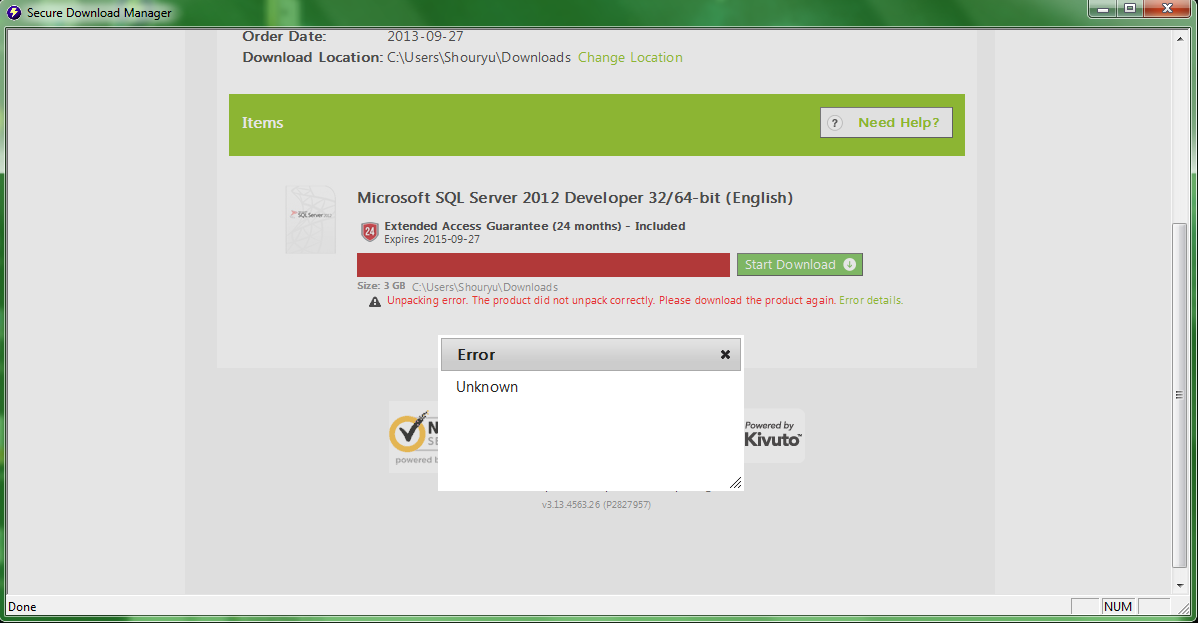
\includegraphics[width=0.8\textwidth]{images/issue00.png}
\caption{SDM error}
\label{fig:SDM_error}
\end{figure}

\subsection{MSSQL}
The installation of MSSQL did not go as smoothly as we had hoped for, we tried to install the MSSQL Management Studio Express first, but this did not install a server instance of the database so we couldn't restore the backup dump we received from the customer. When we had installed a server instance there was problem finding the database dump file - the database dump file needs to be in the correct folders, otherwise the management studio software won't be able to see it. The backup dump was also too big for an express version.

\subsection{ASP.NET Web API}
\label{subsubsec:webapiissues}
During our adaptations of functions from ASP.NET MVC to Web API, we ran into several problems. The first one was that our unfamiliarity with the technology required us to do some testing before we managed to follow the API conventions, which were different from most similiar conventions that we were familiar with.
The next issue was that WebAPIs model binding feature does not play well with Entity Framework classes, something which proved to be the cause of a large amount of time spent troubleshooting.
Finally, we ran into issues with data formatters when Web API was supposed to automatically parse input data from HTTP Request bodies, but didn't, which also was a timesink for troubleshooting and solutions.

\subsection{Naming conventions}
A table in the database was named "System" which collided with the namespace "System" in C\#. This was due to the EF generating a System.cs file which was used instead of the actual System namespace whenever there was a 
\begin{lstlisting}
using System.*;
\end{lstlisting}
statement in our code.

\subsection{\LaTeX}
Most of the group members had previous experience with \LaTeX \ beforehand, though none of us have used it to create as large a report as this current one. Most of us have used sections and subsections, but in this report we needed stuff like subsubsubsections which do not exist in \LaTeX . We also had problems with placing figures/pictures at the correct position in the document, because \LaTeX \ tries to optimize the text and figures so there's less blank space in the document, however this jumbled our ordering of chapters, figures and text. We also had problems with tables to make them appear decent looking.


\subsection{Disk Space}
SSDs tend to be very expensive compared to normal HDD (when comparing cost per byte - however the average SSD are somewhere around 30\% faster than the average HDD). 
Because all of the members in our group have an SSD as their system drive, we experienced problems with limited disk space. Because Windows isn't the main OS for everyone, we had to install it on top of the main OS on some of the computers. Windows 7 needs 30 GiB disk space, and including all the tools needed to get the code up and running (all the development tools and database import etc.) there need to be somewhere around 60 GiB of free space on the disk.

\subsection{File Transferring}
Because the database backup dump was 10.8GiB it was not feasible to download the file via Adressa's server. The customer brought a copy of the file for us on an external USB HDD. We ended up with a copy of the file on one of our computers, but had trouble transferring it to another machine without an external HDD. USB memory sticks were not viable because they are usually less than 10GiB and FAT32 format which has a maximum file size limit of 4GiB. 

\subsection{Construction Work}
The IT building at NTNU has been under construction work since the summer of 2013, and has therefore been affected by a lot of construction noise. This was quite a disturbance when we were attempting to work.

Some of the rooms in the building were also off limits during certain periods, thus limiting our possible workplaces drastically. We were only able to book a room on Wednesdays between the hours of 10 and 14 and Thursdays from 10 to 16, leaving us to search for available rooms whenever we wanted to work together during other time slots.


